\chapter{The Sensory Afferent Database}\label{ch:database}
\graphicspath{{../Figures/50-database/}{figs/50-database/}}

\section{The Resource}\label{sec:sadb_resource}

The Sensory Afferent Database (SADb) is a curated literature resource for studying sensory feedback in locomotion and posture. It connects papers to afferent classes, experimental preparations, feedback pathways, and computational models. I developed it within the AARL's NeuroNex Communication, Coordination, and Control in Nervous Systems (C3NS) effort and presented the resource at Neuroscience 2023 \citep{bolen_sensory_2023}.

SADb addresses the need to recover measured afferent properties, feedback pathways, and experimental conditions from a dispersed literature. Existing reviews organize parts of this evidence \citep{van_de_crommert_review_1998, windhorst_muscle_2007, windhorst_spinal_2022}; the application links individual findings to their sources and candidate controller roles, while distinguishing observations from modeling assumptions.

The primary deliverable is SADb Explorer, a browser application for searching literature records, comparing their classifications, and following groups of papers connected by citations (Figure~\ref{fig:sadb_clusters}). Its embedded snapshot contains 1,393 records, and the table, pivot, and citation views can be used offline. A separate online-search tab identifies candidate additions. The app preserves the collected material independently of the size of the editable curation base, so a reader can inspect both current and archived records.

I used Airtable for editable curation. Linked Papers, Feedback, Models, Review Papers, and Recorders tables supply bibliographic information, source-based notes, classifications, and pathway links. DOI and normalized-title matching reconcile records. SADb Explorer brings these categories together in the distributed application.

\section{Curation Methods}\label{sec:sadb_methods}

The initial collection drew on the literature libraries used for previous AARL papers on locomotion and postural balance, together with records already curated in Airtable. Records were reconciled by DOI and title, then expanded through citation searches. Reviews of spinal and proprioceptive feedback supplied an initial organization of the literature \citep{van_de_crommert_review_1998, windhorst_muscle_2007, windhorst_spinal_2022}. This was a curated research collection, rather than a registered systematic review or an exhaustive search of every relevant publication.

Records were retained when they reported sensory-afferent measurements, investigated feedback in locomotion or posture, or modeled a relevant sensory pathway. Reviews were retained as sources for organizing and locating that evidence. Duplicate records and material outside this feedback scope were removed from the working base. Classification used controlled vocabularies for preparations and afferent classes. Each mechanism summary was grounded in available source text, using the abstract when full text was unavailable; missing text was flagged rather than supplied from recollection.

\section{Results: Application and Corpus Coverage}\label{sec:sadb_corpus}

The application contains 1,393 entries in five record categories: 943 Papers, 247 Models, 157 Review Papers, 42 Feedback pathways, and 4 Recorders. These categories describe how the application organizes the literature and its linked material; they are not a count of unique publications across categories. The table view searches the complete 1,393-entry collection. The pivot and citation views use the 943 entries in the Papers category. Archived records remain searchable in the application. Appendix~\ref{app:sadb_records} records the smaller maintenance subset separately.

Within the application's Papers category, containing 943 entries, 833 carry curation notes, 606 carry animal-preparation tags, 316 carry animal-study assessments, 119 link to feedback pathways, 95 carry an afferent classification, and 363 carry robot-or-simulation translation notes. DOI identifiers are present for 892 papers, and 318 have attached-PDF indicators. These fields overlap and measure the available curation, not independent experimental support. Within that category, 730 papers are connected by 11,130 directed citation pairs, and the Louvain partition resolves 18 named topic clusters. The application distributes the records, citation graph, and cluster assignments together. Figure~\ref{fig:sadb_clusters} illustrates the map; Appendix~\ref{app:sadb_records} shows the table view.



The table view combines text search with filters for preparation, pathway, afferent class, record type, archive status, year, and note or PDF availability (Figure~\ref{fig:sadb_clusters}A). Selecting a record opens its source information, curation notes, and proposed robot-or-simulation translation. The table, pivot, and citation views use the embedded snapshot offline; the separate online-search tab queries OpenAlex for candidate additions and marks DOIs already represented.

The bubble map supports both publication-year versus citation-count axes and a topic landscape based on the citation-network layout. Its controls select the layout, display style, record grouping, citation-neighborhood depth, and click action (Figure~\ref{fig:sadb_clusters}B). Selecting a paper as the focus identifies it in the left panel (C), which exposes its curation note and proposed robot-or-simulation translation (D). The plotted neighborhood can extend through one, two, or three citation links in either direction (E). Direct connections retain color, while more distant papers are gray. In the illustrated Grillner (1985) neighborhood, 57 in-corpus papers cite the focus, the focus cites 13 in-corpus papers, and 555 papers lie within two links. Green triangles identify incoming citations and red circles identify the focus paper's references. These synapse-like symbols encode bibliographic direction; they do not assert excitatory or inhibitory physiological effects.

The connection list separates papers citing the focus from its references (Figure~\ref{fig:sadb_clusters}F). Selecting a listed paper makes it the new focus, allowing a reader to follow the development of an idea without repeatedly searching for individual titles. The reference-only and cited-by views isolate either direction, and the detail action opens the underlying record. A researcher can therefore start from a known experiment, inspect earlier studies supporting it, follow subsequent models or experiments citing it, and read the associated translation notes before choosing a candidate pathway for simulation.

\begin{sidewaysfigure}[p]
\centering
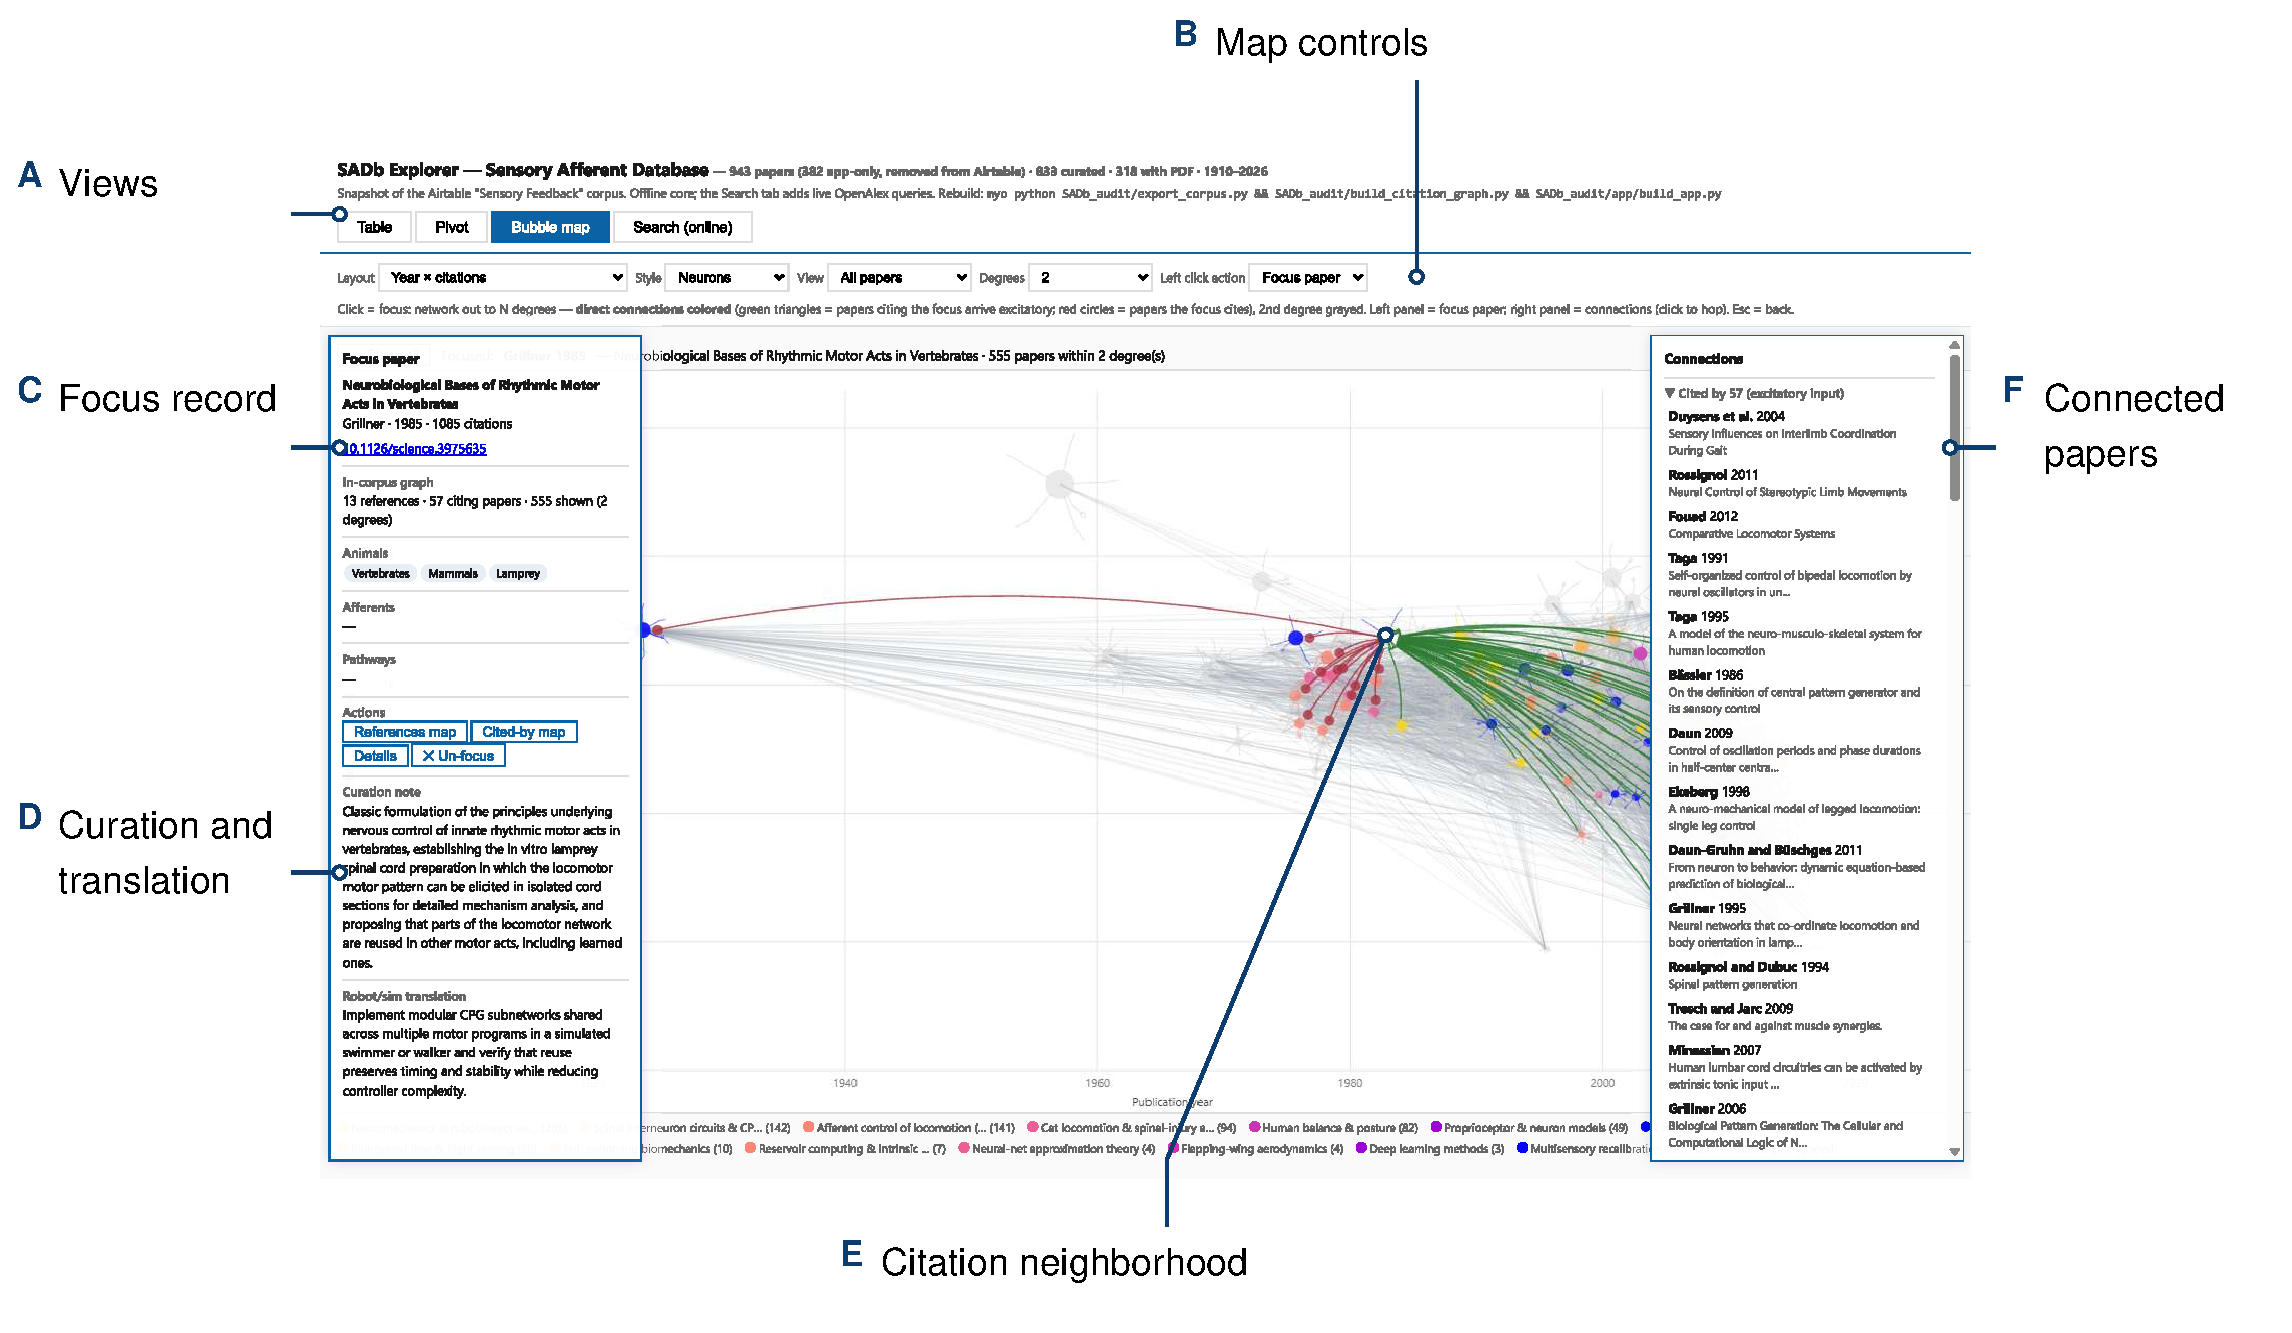
\includegraphics[width=\linewidth]{sadb_bubble.pdf}
\caption[SADb Explorer citation-map functions]{SADb Explorer focused on Grillner (1985): views (A), map controls (B), focus record (C), curation and translation notes (D), citation neighborhood (E), and connected papers (F).}
\label{fig:sadb_clusters}
\end{sidewaysfigure}

\subsection{AI-Assisted Literature Triage}\label{sec:sadb_triage}

I evaluated AI-assisted literature identification, summarization, and categorization in work presented at Neuroscience 2024 \citep{bolen_using_2024}. The comparison included ResearchRabbit, Litmaps, txyz, SciSpace, and MirrorThink. Some tools helped identify related papers or summarize straightforward material, but categorization remained inadequate: none received a good rating, and only txyz was rated adequate. Complex models and nuanced physiological findings required substantial human correction. The tools therefore offered limited help with the central curation task of accurately assigning papers to database categories. I retained responsibility for inclusion, classification, and deletion decisions after checking the source.

\section{Discussion}\subsection{Robot and Simulation Use}\label{sec:sadb_use}

SADb supports sensory-pathway selection for Chapter~\ref{ch:sns}. Its afferent and pathway tables connect candidate signals, connection signs, and phase dependence to the cited evidence (Tables~\ref{tab:sadb_afferents} and~\ref{tab:sadb_pathways}). Receptor dynamics, gains, delays, and species-specific assumptions still require explicit selection and testing. The model records connect proposed implementations to their literature, including two-level rhythm generation and pattern formation \citep{rybak_modelling_2006}, muscle-reflex walking \citep{geyer_musclereflex_2010}, and the laboratory walker lineage \citep{deng_neuromechanical_2019}.



The pivot view counts papers by two selected dimensions, including topic cluster, decade, primary author, animal preparation, feedback pathway, and afferent classification. Figure~\ref{fig:sadb_pivot} crosses afferent classes with animal preparations: each cell counts papers carrying both tags. Rows and columns can be ordered alphabetically or by count. Selecting a cell opens the corresponding records in the table view, and a return control restores the pivot. The pivot is computed over the 943 entries in the Papers category, including archived entries, rather than all 1,393 records. Because a paper can carry several animal or afferent tags, it can contribute to several cells. The counts describe the distribution of curated records, not independent experimental observations or the strength of evidence for a pathway.

\begin{figure}[htbp]
\centering
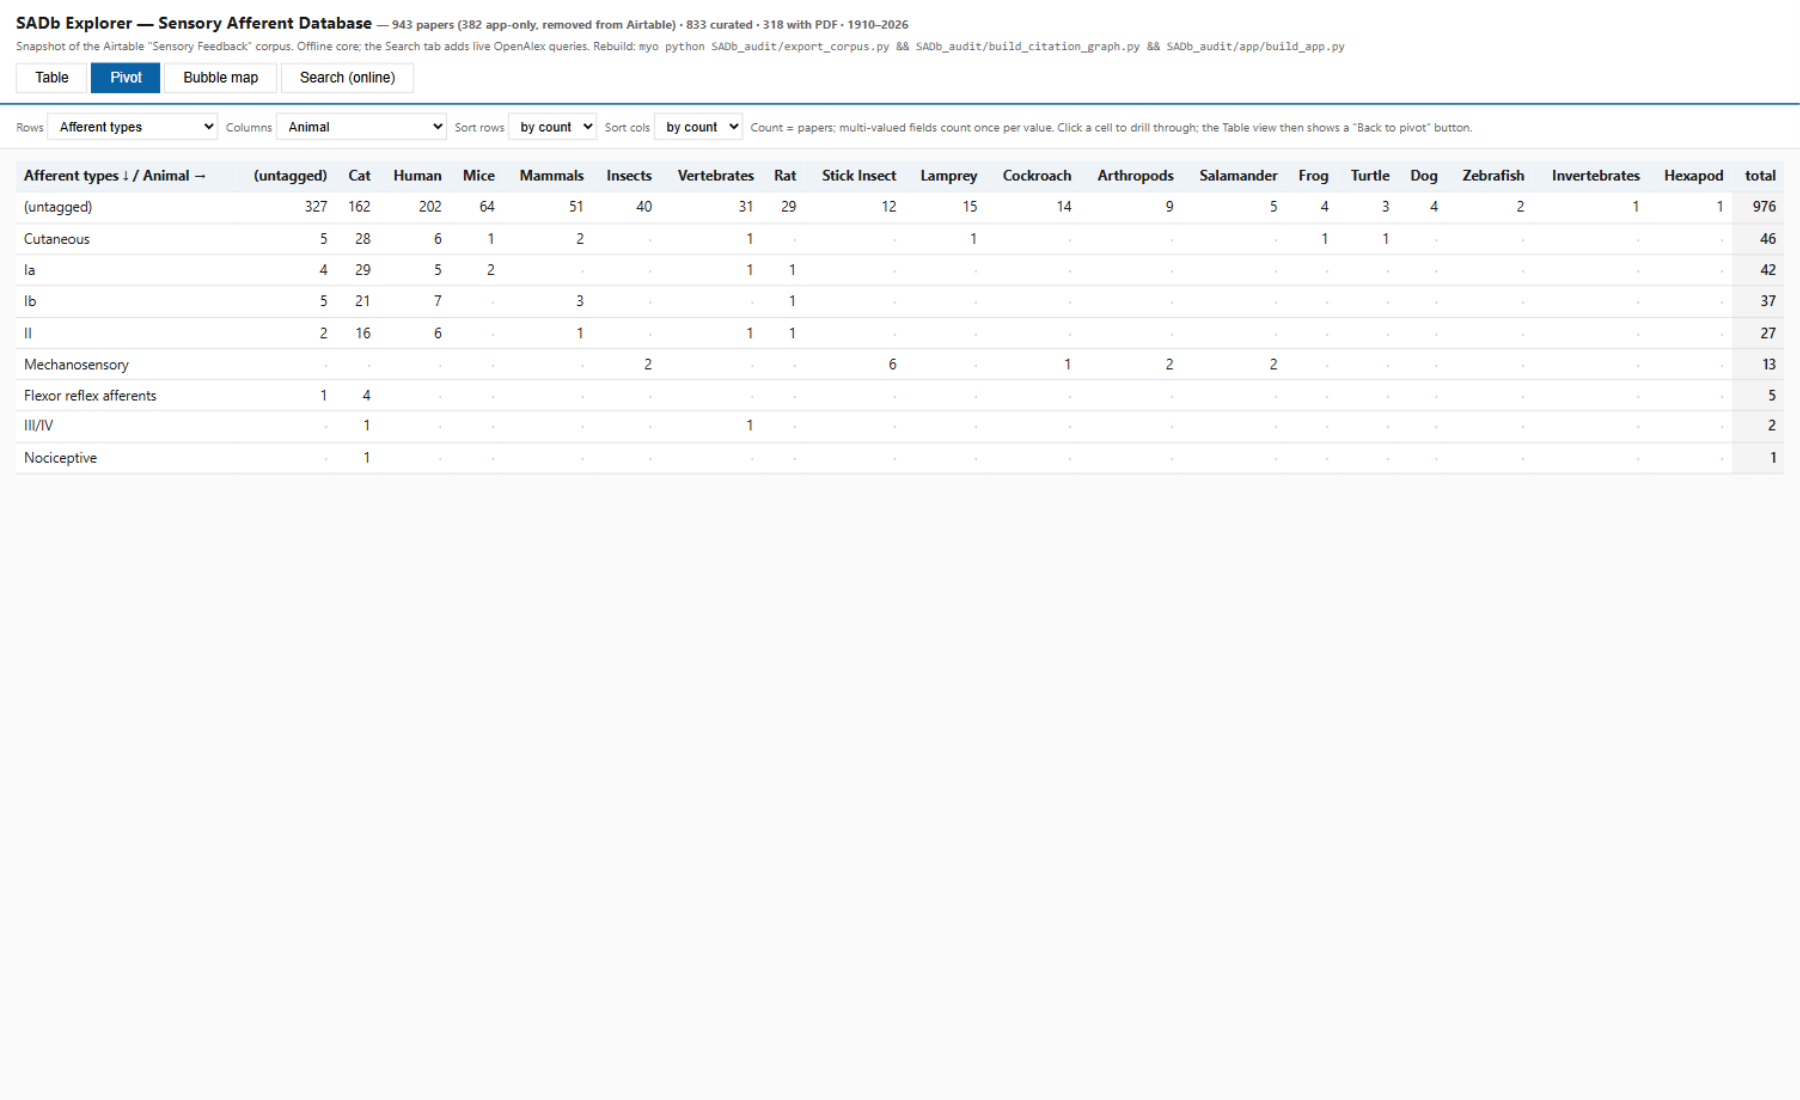
\includegraphics[width=0.96\textwidth]{sadb_pivot_app.png}
\caption[The SADb Explorer pivot view]{SADb Explorer pivot table by afferent classification and animal preparation. Each cell counts papers carrying both tags and links to those records.}
\label{fig:sadb_pivot}
\end{figure}



The feedback-pathway records extend beyond the mammalian core of Table~\ref{tab:sadb_pathways}: paired excitation and inhibition records cover the chordotonal organs and trochanteral hair plates of insect legs, a load-feedback record covers the campaniform sensilla, and further records hold fictive locomotion without sensory feedback (12 linked papers), group III/IV fatigue, and one paper each for somatosensory, vestibular, and visual contributions to postural control. The controller of Chapter~\ref{ch:sns} implements the mammalian subset.

The balance, posture, and multisensory-recalibration clusters provide entry points for the vestibular and visual extensions proposed in Section~\ref{sec:fw_senses}. Preparation-based searches also let new users approach the literature through the experiment they intend to perform.

\subsection{Further Improvements}

Classification remains incomplete within the application's 943-entry Papers category: 95 carry an afferent classification, and 119 link to named pathways. Completing these fields would improve comparisons across preparations and help expose where a proposed pathway depends on a small or indirect body of evidence. Missing source text should remain explicit until the paper can be checked; model and review records should link to the primary experiments supporting their assumptions.

Further curation should connect pathway records to the papers that establish their signals, connection signs, and task dependence, and connect model records to the pathways they implement. Vestibular and visual contributions to posture require expanded classifications and source coverage before the database can support the additional sensory channels proposed in Section~\ref{sec:fw_senses}. New records should include a source identifier and a substantive curation note, with incomplete classifications flagged for review. These improvements would make the resource more useful for selecting experiments and constructing testable neural models.


The application makes physiological evidence accessible for controller design, but selecting a pathway is only the beginning of a neuromechanical experiment. Its encoding, connection sign, gain, and interaction with the body must still be implemented and tested. Chapter~\ref{ch:sns} develops the models and simulation tools needed to make that next step explicit.
